\documentclass[11pt]{article}
\usepackage[letterpaper,margin=1in]{geometry}
\usepackage[T1]{fontenc}
\usepackage{lmodern}
\usepackage{amsmath,amssymb}
\usepackage{graphicx}
\usepackage{booktabs}
\usepackage{tabularx}
\usepackage{caption}
\usepackage{tikz}
\usetikzlibrary{calc}
\usepackage[hidelinks]{hyperref}
\captionsetup{font=small,labelfont=bf}

\begin{document}

\begin{center}
{\Large\bfseries How Lizards Become Snake-like:\\[2pt] A Plain-Language Guide to Our Network Study of Evolution}\\[8pt]
Henry Ji and Calvin Zhang\\
CS/INFO 6850, Structure of Information Networks, November 2026
\end{center}

\vspace{6pt}
\noindent This paper explains our course project for a reader who knows nothing about evolution or graph algorithms. We start with the puzzle that motivates the project and the questions we ask. Then we introduce the few ideas from biology and from network science that the project needs, describe the data and the model, walk through each graph algorithm and what it tells us, and end with the big picture. A glossary at the end collects the technical terms.

\section{The puzzle}

Lizards come in a huge variety of shapes, but most share the same basic design: a short body carried on four legs, each ending in five fingers or toes. A small minority look completely different. Their bodies are long and thin, their legs are tiny stubs or are missing entirely, and many of them live underground. They look like snakes, but they are lizards. Australian sand-swimming skinks, European glass lizards, the legless lizards of South America and the burrowing ``worm lizards'' all belong to this group. Snakes themselves are the most famous example, but they are only one of many.

What makes this interesting is that these snake-like lizards are not close relatives of each other. The snake-like body has been invented over and over again, independently, in families that split apart tens or hundreds of millions of years ago. Biologists call this \emph{convergent evolution}: unrelated lineages arriving at the same design on their own, the way birds and bats each evolved wings.

This creates a puzzle. The snake-like body is rare: in our data only about one lizard species in seven has it. Yet it keeps reappearing. If the body is hard to evolve, why has it evolved dozens of times? If it is easy, why is it not common? Our project uses the mathematics of networks to look at this puzzle from a new angle.

\section{The questions we are answering}

We ask four questions, each answered with a different tool (Table~\ref{tab:questions}). The first is about place: when unrelated lineages converge on the snake-like body, is there a single narrow passage they all go through, and who sits in it? The second is about time: which steps of the transformation are slow and which are fast? The third is about direction: does evolution have a tendency to move toward the snake-like body, and how strong is it? The fourth is about causes: which living conditions push lizards in this direction, and what would happen if those conditions changed? For every answer we also ask how sure we can be.

\begin{table}[h]
\centering
\small
\begin{tabularx}{\textwidth}{@{}lXl@{}}
\toprule
Question & In plain words & Main tool \\
\midrule
1. Convergence & Where do unrelated lineages end up, and through what passage? & Cheeger cut on a species network \\
2. Time & Which steps take a long time, and which happen quickly? & Model of change on the family tree \\
3. Direction & Which way does evolution lean, and how strongly? & Biased random walks \\
4. Causes & What pushes lizards toward a snake-like body? What if conditions changed? & Fitted drivers and what-if scenarios \\
\bottomrule
\end{tabularx}
\caption{The four questions and the tools we use to answer them.}
\label{tab:questions}
\end{table}

Our contribution is not a new theory of evolution. It is a new way of looking at existing data: we turn species into a network and use the tools of network science, the subject of this course, to read off where evolution converges, where it stalls and which way it flows.

\section{Two ideas we need}

\subsection{Evolution and family trees}

Every species changes slowly over many generations, because individuals whose bodies suit their surroundings leave more offspring. From time to time one species splits into two, and from then on each branch changes on its own. A \emph{lineage} is one line of descent through time, like a single path from an ancestor down to one living species.

Because species split, all living species are connected by a family tree, which biologists call a \emph{phylogeny}. The tips of the tree are species alive today, the branching points are ancestors where one species split into two, and the length of each branch is the time that passed. Scientists build these trees from DNA, and modern trees are dated, so we know roughly when each split happened. We use a tree of 6,885 species of lizards and snakes (Title et al.\ 2024). One important limitation runs through the whole project: we can see and measure living species, but we cannot see the ancestors. What the ancestors looked like has to be inferred.

Figure~\ref{fig:toys}a shows a small made-up tree. Two of its six species have become snake-like, but they sit on distant branches, so each must have become snake-like on its own. That is convergence.

\begin{figure}[t]
\centering
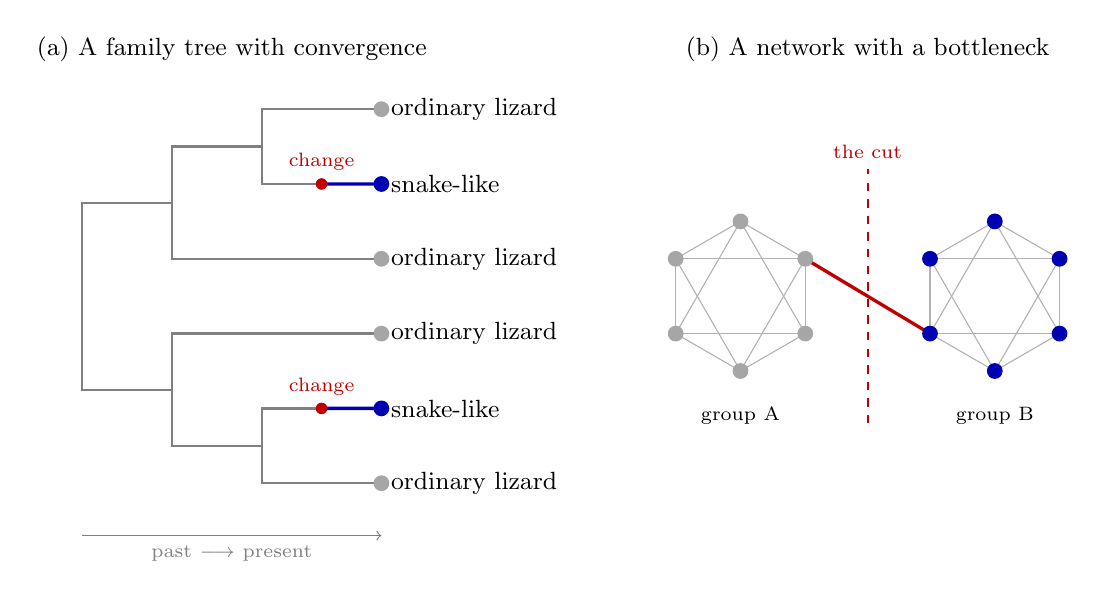
\begin{tikzpicture}[scale=0.95, every node/.style={font=\small}]
% (a) toy family tree
\begin{scope}
\coordinate (r) at (0,2.5);
\coordinate (n2) at (1.2,3.75);
\coordinate (n1) at (2.4,4.5);
\coordinate (n4) at (1.2,1.25);
\coordinate (n3) at (2.4,0.5);
\foreach \i/\y in {1/5,2/4,3/3,4/2,5/1,6/0} { \coordinate (t\i) at (4,\y); }
\draw[thick, gray] (r) |- (n2); \draw[thick, gray] (r) |- (n4);
\draw[thick, gray] (n2) |- (n1); \draw[thick, gray] (n2) |- (t3);
\draw[thick, gray] (n1) |- (t1); \draw[thick, gray] (n4) |- (t4); \draw[thick, gray] (n4) |- (n3);
\draw[thick, gray] (n3) |- (t6);
\draw[thick, gray] (n1) |- (3.2,4); \draw[very thick, blue!70!black] (3.2,4) -- (t2);
\draw[thick, gray] (n3) |- (3.2,1); \draw[very thick, blue!70!black] (3.2,1) -- (t5);
\fill[red!75!black] (3.2,4) circle (2.2pt); \fill[red!75!black] (3.2,1) circle (2.2pt);
\foreach \i in {1,3,4,6} { \fill[gray!70] (t\i) circle (3pt); \node[right] at (t\i) {ordinary lizard}; }
\foreach \i in {2,5} { \fill[blue!70!black] (t\i) circle (3pt); \node[right] at (t\i) {snake-like}; }
\node[red!75!black, above] at (3.2,4.05) {\scriptsize change};
\node[red!75!black, above] at (3.2,1.05) {\scriptsize change};
\draw[->, gray] (0,-0.7) -- (4,-0.7) node[midway, below] {\scriptsize past $\longrightarrow$ present};
\node at (2,5.8) {(a) A family tree with convergence};
\end{scope}
% (b) toy bottleneck graph
\begin{scope}[xshift=8.8cm, yshift=2.5cm]
\foreach \a [count=\i] in {90,150,210,270,330,30} { \coordinate (L\i) at ($(0,0)+(\a:1.0)$); \coordinate (R\i) at ($(3.4,0)+(\a:1.0)$); }
\foreach \i/\j in {1/2,2/3,3/4,4/5,5/6,6/1,1/3,2/4,3/5,4/6,5/1,6/2} { \draw[gray!60] (L\i) -- (L\j); \draw[gray!60] (R\i) -- (R\j); }
\draw[very thick, red!75!black] (L6) -- (R3);
\foreach \i in {1,...,6} { \fill[gray!70] (L\i) circle (3pt); \fill[blue!70!black] (R\i) circle (3pt); }
\draw[dashed, red!75!black, thick] (1.7,-1.7) -- (1.7,1.7) node[above] {\scriptsize the cut};
\node at (0,-1.6) {\scriptsize group A}; \node at (3.4,-1.6) {\scriptsize group B};
\node at (1.7,3.3) {(b) A network with a bottleneck};
\end{scope}
\end{tikzpicture}
\caption{(a) A made-up family tree of six species. Time runs left to right. Two distant species have each become snake-like (blue), so the snake-like body evolved twice, independently (red dots). (b) A made-up network: two tightly knit groups joined by a single link. Cutting that one link splits the network in two, so the link is a bottleneck. Finding such cuts in large networks is what the Cheeger method does.}
\label{fig:toys}
\end{figure}

\subsection{Networks, also called graphs}

A \emph{network}, which mathematicians call a \emph{graph}, is simply a set of dots joined by lines. The dots are called \emph{nodes} and the lines \emph{edges}. Two nodes joined by an edge are \emph{neighbors}, and a \emph{path} is a sequence of edges that leads from one node to another. A road map is a graph (towns joined by roads), and so is a social network (people joined by friendships). Edges can also carry \emph{weights}, numbers that say how strong a connection is. Network science studies the shape of such graphs: whether they have tight clusters, how many steps it takes to get from anywhere to anywhere, and where they are thin or fragile. Figure~\ref{fig:toys}b shows a small graph with an obvious weak point.

\section{The data}

For each species we need a few simple facts about its body. We use three. The first is the number of \emph{presacral vertebrae}, the backbone bones between the head and the hips. A longer, more snake-like body has more of them: an ordinary lizard has about 26, a snake-like lizard 40 to over 100, and some snakes more than 300. We checked that this count really measures body shape: in 231 species with direct measurements it tracks the ratio of body length to body width closely (rank correlation 0.87) and runs opposite to limb length ($-0.89$). The second fact is the number of fingers and toes, counted on one side of the body, so a fully limbed lizard has 10. The third is whether the species lives underground, burrowing through soil or sand.

We combined five scientific datasets that each cover part of this information: a 2025 compilation of digits, vertebrae and habitats for 1,386 species, vertebral counts for 2,364 species taken mostly from X-ray images of museum specimens, a database of all known skinks with reduced limbs (Camaiti et al.\ 2022), body measurements from Bergmann and Morinaga (2019), and SquamBase (Meiri 2024), which lists basic traits for every one of the 11,744 known lizard and snake species. Where two sources measured the same species we compared them, and they agreed almost perfectly: vertebral counts correlated at 0.99 across 1,052 species, and finger and toe counts at 0.98. Where no source counted fingers and toes, we filled in 10 for species described as having ``four well developed limbs,'' which is correct 96\% of the time where we can check it. In the end we have 2,403 species with both counts. Of these, 1,451 are lizards and 952 are snakes. We leave snakes out of the species network, because all snakes descend from a single snake-like ancestor and so count as one invention of the body, but we keep them in the evolutionary model.

\section{The model of evolution}

\subsection{A map of body plans}

To talk about how bodies change, we describe each body with four yes-or-no features: is it elongate (35 or more vertebrae), has it lost some fingers or toes, has it lost all of them, and does it burrow? We abbreviate these E, R, Z and F. Every species is then one combination of answers, which we call a \emph{body plan}. Four yes-or-no features give 16 combinations, but four of them are impossible, because a lizard cannot have lost all its digits without having lost some, so 12 body plans remain.

These body plans form a graph of their own, a map of possible bodies (Figure~\ref{fig:bodyplans}). Two body plans are neighbors if they differ in exactly one feature, so moving along an edge means gaining or losing one feature. The ordinary lizard sits at one corner, with none of the four features, and the fully snake-like burrower sits at the opposite corner, with all four. Mathematicians call this kind of graph a \emph{hypercube}, here with a few corners removed.

\begin{figure}[t]
\centering
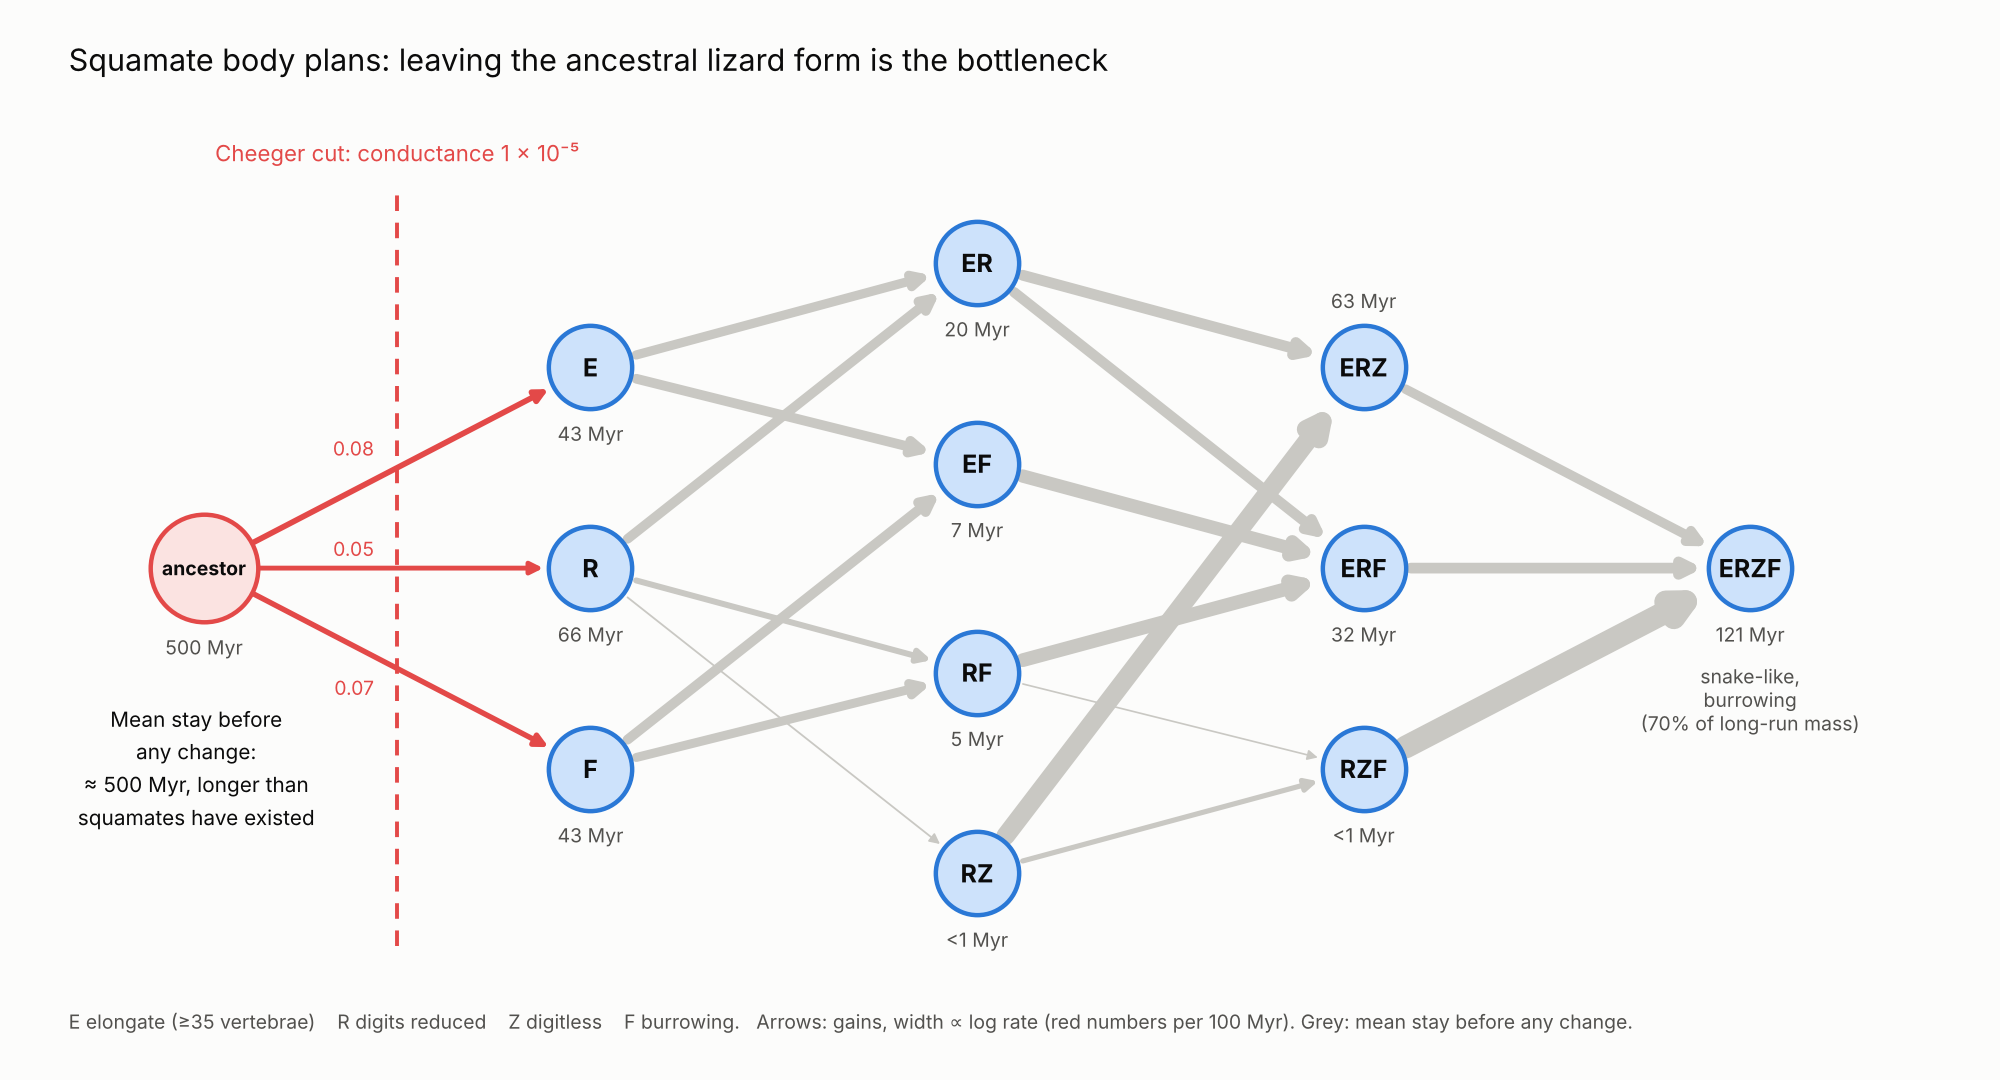
\includegraphics[width=\textwidth]{figures/bodyplans.png}
\caption{The map of body plans. Each circle is a body plan, named by the features it has (E elongate, R digits reduced, Z no digits, F burrowing); arrows are single gains, thicker when the fitted rate is higher. The number under each circle is how long a lineage typically stays in that body plan before changing. The ordinary lizard (left) stays about 500 million years, far longer than any other body plan; the dashed line is the bottleneck the Cheeger method finds on this map.}
\label{fig:bodyplans}
\end{figure}

\subsection{How a lineage moves on the map}

Picture each lineage as a token sitting on one circle of the map. As time passes along a branch of the family tree, the token occasionally hops to a neighboring circle: the lineage gains or loses one feature. When the species splits, the token is copied, and the two copies continue independently down the two new branches. The hops happen at random moments, but each kind of hop has its own \emph{rate}: how often, on average, it happens per million years. This kind of process, where what happens next depends only on where you are now and not on how you got there, is called a \emph{Markov chain}. It is the standard way biologists model the evolution of yes-or-no features (Pagel 1994).

The key ingredient is that rates can depend on the features a lineage already has. Having a long body might, for example, make it much easier to lose the toes. We capture this with one number for each ordered pair of features, which says how many times faster feature B is gained when the lineage already has feature A. These \emph{dependencies} are exactly what lets one change make the next one easier, and they are estimated from the data rather than assumed.

\subsection{Fitting the model to the data}

The model has 15 adjustable numbers: four basic rates of gaining each feature, one rate of losing features, and ten dependencies. Any choice of these numbers is a different story about how evolution worked. For each story we can compute how probable it makes the features we actually observe in the 6,885 living species. This probability is called the \emph{likelihood}, and \emph{fitting} the model means searching for the 15 numbers that make the likelihood as large as possible.

Computing the likelihood requires accounting for every possible appearance of every unseen ancestor, which naively is an astronomical number of combinations. Felsenstein's algorithm makes it fast, and it is itself a graph algorithm on the family tree. It works from the tips toward the root: at each branching point it combines what the two branches below say about the possible states of the ancestor, so each ancestor is handled once and the total work grows only in proportion to the size of the tree.

Once the model is fitted, we use it to generate complete, plausible histories of every lineage that agree with what we see today, a method called \emph{stochastic mapping} (Nielsen 2002). Each history says when each feature was gained or lost along every branch. We generate many such histories and average over them. From them we can count how many separate times the snake-like body evolved and time each step.

\section{The graph ideas at play}

\subsection{Building the species network}

Our main network has one node per lizard species. We connect each species to two kinds of neighbors. Its six closest relatives are the species whose lineages split from it most recently on the family tree. Its six closest look-alikes are the species with the most similar numbers of fingers, toes and vertebrae. Connecting each node to its $k$ nearest neighbors in this way is a standard construction called a \emph{$k$-nearest-neighbor graph}, here with $k = 6$. Most look-alike edges join relatives that resemble each other because they inherited the same body. The interesting ones join unrelated species: we call a look-alike edge a \emph{convergence link} when both species have a derived, snake-ward body and their lineages split more than 100 million years ago. These are the network's record of convergent evolution.

\subsection{Small worlds}

In many real networks, from friendships to power grids, two properties appear together. Nodes are \emph{clustered}: your neighbors tend to be neighbors of each other. And yet \emph{paths are short}: you can reach almost anyone in a few steps. Watts and Strogatz (1998) explained this combination, which they named a \emph{small world}. A network made only of local, clustered connections has long paths, but adding a few random long-range shortcuts collapses the distances while leaving the clustering intact. The famous ``six degrees of separation'' is an example.

We measure clustering with the \emph{clustering coefficient}, the fraction of a node's pairs of neighbors that are themselves connected, and distance with the average number of steps between nodes. We compare both with a \emph{random graph}, in which the same number of edges is placed completely at random.

\subsection{Bottlenecks and the Cheeger cut}

A \emph{bottleneck} is a place where a network is thin: a way of splitting the nodes into two groups so that few edges cross between them, compared with how many edges each group has (Figure~\ref{fig:toys}b). The standard measure of thinness is \emph{conductance}. For a split of the nodes into a group $S$ and the rest,
\[
\text{conductance}(S) = \frac{\text{total weight of the edges crossing between } S \text{ and the rest}}{\text{total weight of the edges touching the smaller side}},
\]
so a conductance near 0 means a near-complete separation and a conductance near 1 means no bottleneck at all.

Finding the split with the lowest conductance is very hard in general. With 1,451 species there are about $2^{1451}$ ways to split them, far too many to try, and no known fast method finds the exact best split. The \emph{spectral method} finds a good one quickly. It computes a special list of numbers called the \emph{second eigenvector of the graph Laplacian}, or \emph{Fiedler vector}, which assigns one number to each node. An intuition is to imagine heat spreading across the network: the Fiedler vector describes the pattern that evens out most slowly, and it evens out slowly exactly because heat has trouble crossing a bottleneck, so nodes on the same side of a bottleneck get similar numbers. We sort the nodes by their numbers and check every split along that order, a \emph{sweep cut}, keeping the one with the lowest conductance. \emph{Cheeger's inequality}, a classic theorem of spectral graph theory (Chung 1997), guarantees that this split is never far from the best possible one.

For this question we use a version of the network built from body shape alone, in which every pair of species is linked with a weight that is large when their bodies are similar and fades quickly as they differ. The question is then where body-shape space is thinnest. Afterwards we use the family tree to ask who sits on each side: if one side contains many unrelated families, then many separate lineages have converged on it. The species whose edges carry most of the weight across the cut are the \emph{bridge species}, the in-between forms that connect the two sides.

\subsection{Random walks}

A \emph{random walk} on a graph is a wanderer that starts at some node and, at each step, moves to a neighbor chosen at random. Random walks are a central tool of network science because they reveal structure: a walker gets stuck on one side of a bottleneck for a long time, and the long-run fraction of time it spends at each node, called the \emph{stationary distribution}, shows where the network ``pulls'' it. The \emph{hitting time} is the expected number of steps the walker needs to reach a given set of nodes.

An unbiased walker picks each neighbor with equal chance, so its behavior reflects only the shape of the network. Evolution, however, may lean one way. We measure the lean directly from the reconstructed histories: for each feature, how many times more often it was gained than lost. We then build a \emph{biased walk} in which steps that gain a feature are favored by those observed ratios and steps that lose one are disfavored, like a wanderer on a gently sloping floor. Comparing the biased and unbiased walkers separates evolution's direction from the shape of the network.

The same ideas apply to the map of body plans in Figure~\ref{fig:bodyplans}, because the evolutionary model is itself a random walk on that map: each lineage's history is a walk from body plan to body plan. On that map the time a lineage spends in a body plan before moving on is its \emph{mean stay}, and a long mean stay marks a slow step.

\subsection{Drivers and what-if scenarios}

To find out which living conditions push lizards toward a snake-like body, we add the environment to the model as one more yes-or-no feature that also changes along the family tree: does the lineage live underground, in a desert or in a tropical rainforest? We fit dependencies in both directions, so the model can tell apart two different stories: ``living in this environment makes the body change faster'' and ``lizards with this body tend to move into this environment.'' Only the first is a driver. A \emph{what-if scenario} then changes one thing, such as how often lineages take up burrowing, keeps every fitted number fixed, and asks how much the expected time to a snake-like body changes.

\section{What we found}

\begin{figure}[t]
\centering
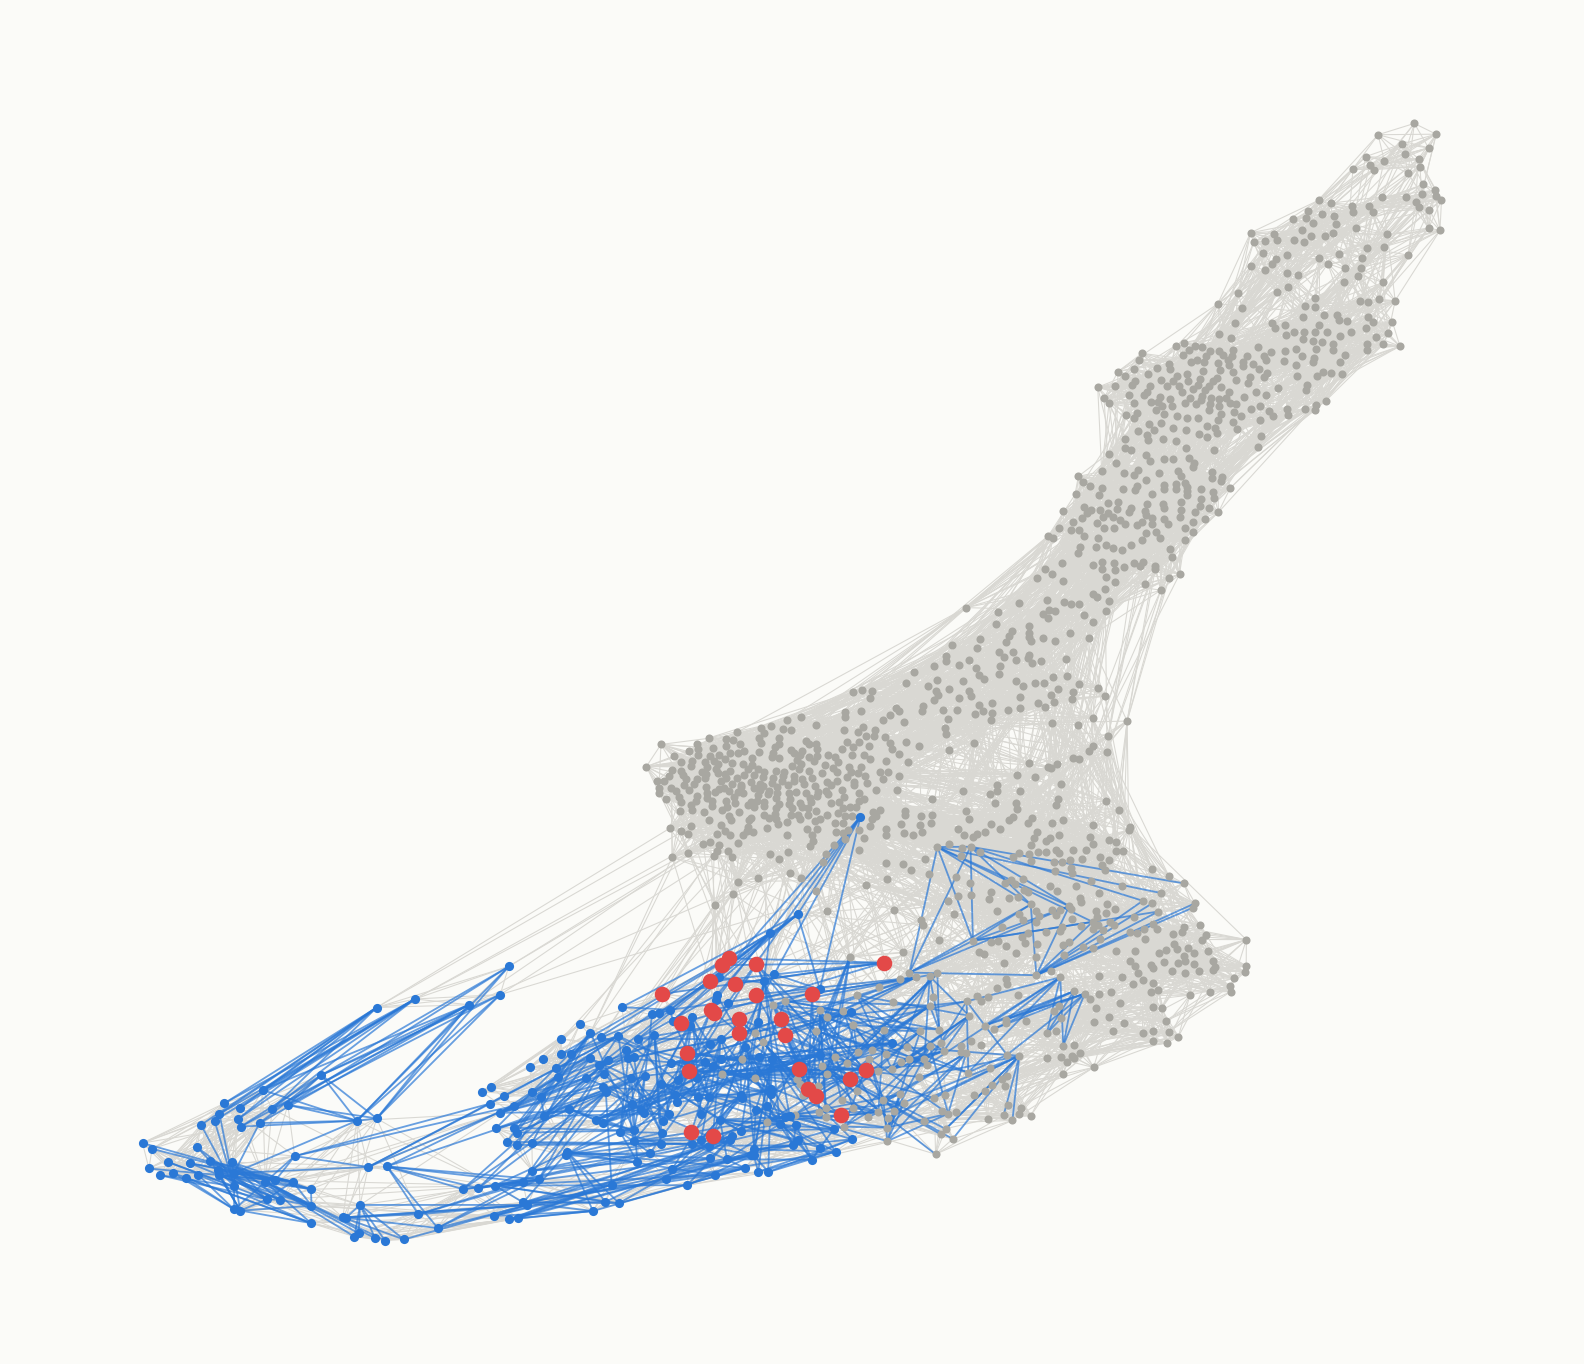
\includegraphics[width=0.4\textwidth]{figures/network.png}\hfill
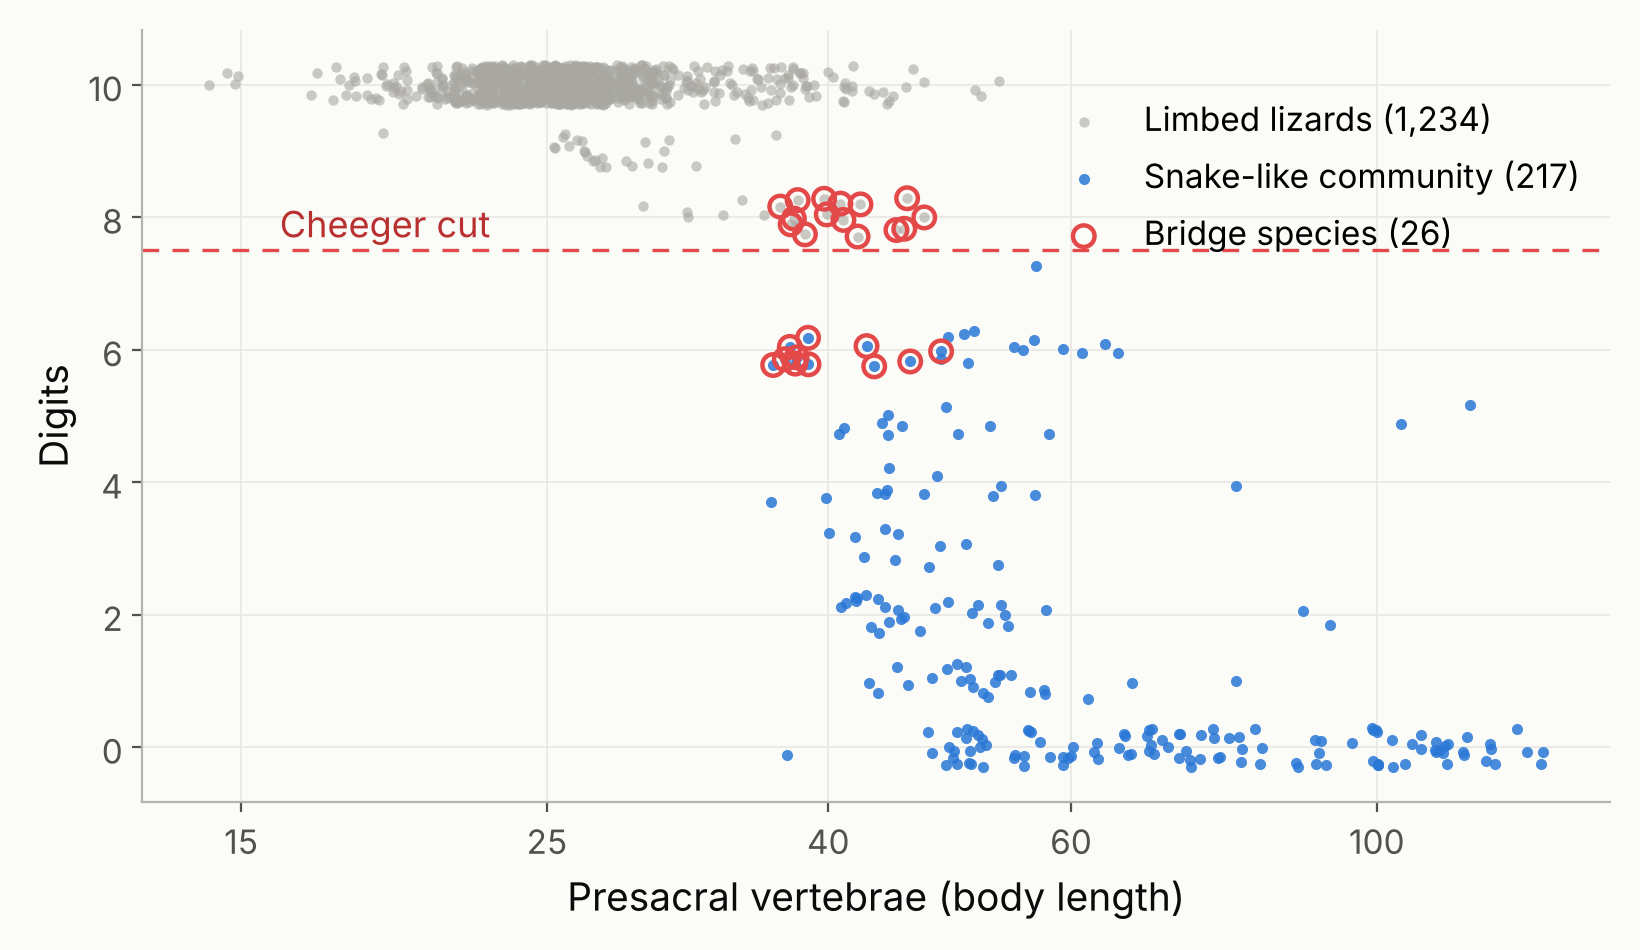
\includegraphics[width=0.56\textwidth]{figures/cut.png}
\caption{Left: the species network of 1,451 lizards, laid out so that connected species sit close together. Grey nodes are ordinary limbed lizards, blue nodes the snake-like side of the bottleneck, blue edges convergence links between unrelated species, and red nodes the bridge species. Right: the same species placed by vertebrae and digits. The dashed line is the bottleneck: ordinary lizards above, snake-like lizards below, and very few species in between.}
\label{fig:network}
\end{figure}

\subsection{The network is a small world held together by convergence}

If we connect species only to their relatives, the network falls apart into 45 separate pieces, one for each group of related species. The look-alike edges reconnect everything into a single network. The result is a small world: clustering is 18 times higher than in a random graph with the same number of edges, while the average path is only 1.39 times longer. The 720 convergence links, joining snake-ward species whose lineages split over 100 million years ago, play the role of Watts and Strogatz's long-range shortcuts.

\subsection{Question 1: one narrow passage, many separate lineages}

The Cheeger method finds a single, very sharp bottleneck in body-shape space (Figure~\ref{fig:network}). Its conductance is 0.003, compared with 0.38 for the best split anywhere among ordinary lizards, so it is more than a hundred times thinner than anything else in the network. On one side are 1,234 ordinary four-legged lizards. On the other are 217 snake-like lizards from 15 different families and about 30 lineages that separated more than 50 million years ago. Many separate lineages have converged on the same region of the network. Only 26 species sit on the bridge between the two sides, with bodies in between: a few digits missing and a moderately long trunk. They belong to genera such as \emph{Lerista}, \emph{Brachymeles}, \emph{Bachia}, \emph{Hemiergis} and \emph{Chalcides}, which biologists already study as textbook examples of limb loss. The method found them without being told.

\subsection{Question 2: hard to start, quick to finish}

The reconstructed histories show why the bridge is so empty. A typical ordinary lizard lineage waits about 510 million years before any change toward the snake-like body begins. That is longer than lizards and snakes have existed (about 206 million years), which means most lineages never start at all. Once a lineage does start, it reaches the snake-like body in about 36 million years. In-between forms are rare because lineages pass through them quickly instead of settling there. The snake-like body evolved about 47 separate times, and in about 71\% of cases the body lengthened before any fingers or toes were lost.

The fitted dependencies explain the speed of the second phase. Burrowing makes elongation and toe loss about 16 times faster, a long body and reduced toes each make the other 14 to 18 times faster, and a long body makes the complete loss of digits at least 400 times faster. Each change makes the next one easier, so once the first step happens the rest follow like a snowball rolling downhill. On the map of body plans this shows up as a bottleneck around the ordinary lizard itself (Figure~\ref{fig:bodyplans}): getting started is the hard part.

\subsection{Question 3: evolution leans toward the snake-like body}

Every one of the four features was gained more often than it was lost, by factors between 1.9 and 7.1. A random walker on the species network that follows these real tendencies reaches the snake-like side in about 60 steps, against about 156 for an unbiased walker, a speedup of 2.6 times (Figure~\ref{fig:walks}). In the long run the biased walker spends most of its time on the snake-like side, which acts like a basin that evolution drains toward.

\begin{figure}[t]
\centering
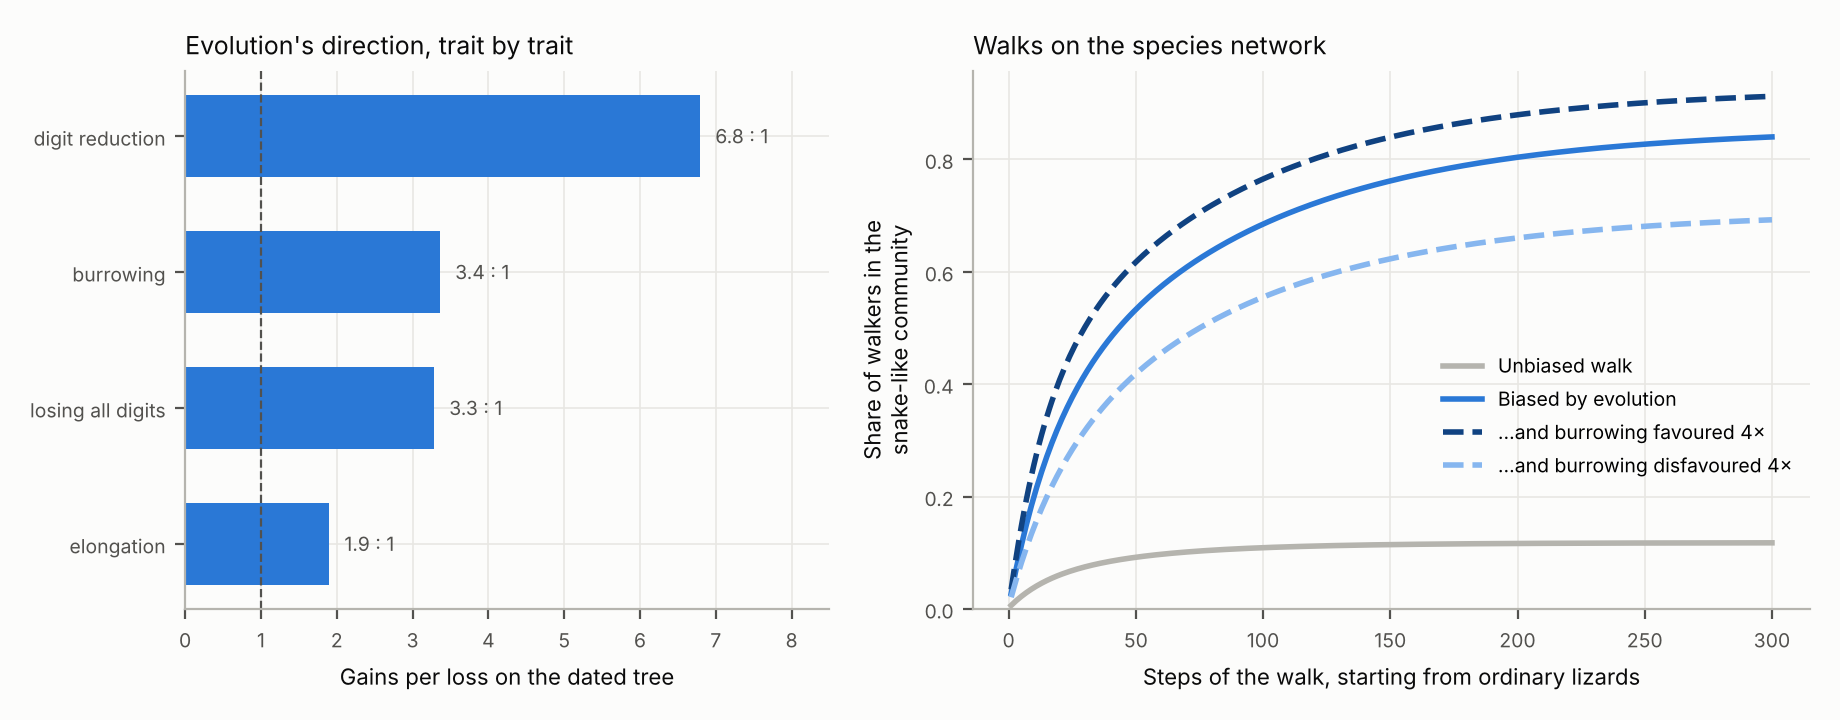
\includegraphics[width=0.98\textwidth]{figures/walks.png}
\caption{Left: how many times more often each feature was gained than lost in the reconstructed histories. Right: the share of random walkers that have reached the snake-like side, starting from ordinary lizards. The walker that follows evolution's observed tendencies (solid blue) gets there far faster than an unbiased walker (grey). The dashed lines repeat the biased walk with burrowing made four times more or less favored.}
\label{fig:walks}
\end{figure}

\subsection{Question 4: burrowing is the push}

Of the environments we tested, only living underground drives the change (Figure~\ref{fig:drivers}). Burrowing lineages lengthen their bodies and lose digits about 16 times faster than others. Deserts and tropical rainforests do not speed up any body change. Their relationship runs the other way: lizards that are already long-bodied tend to move into deserts, and lineages that have lost their digits tend to move into rainforests. This distinction matters, because a simple correlation between habitat and body shape cannot tell cause from consequence, while the model can.

The what-if scenarios use only these fitted numbers. If lizard lineages took up burrowing twice as often, as might happen if surface habitats were lost and animals were pushed underground, snake-like bodies would appear about 25\% sooner. If burrowing became half as common, for instance because soils became degraded or polluted, they would appear about 24\% later. Doubling how often lineages enter or leave deserts or rainforests changes the answer by at most 7\%. These are thought experiments about the patterns in the data, not forecasts of the future.

\begin{figure}[t]
\centering
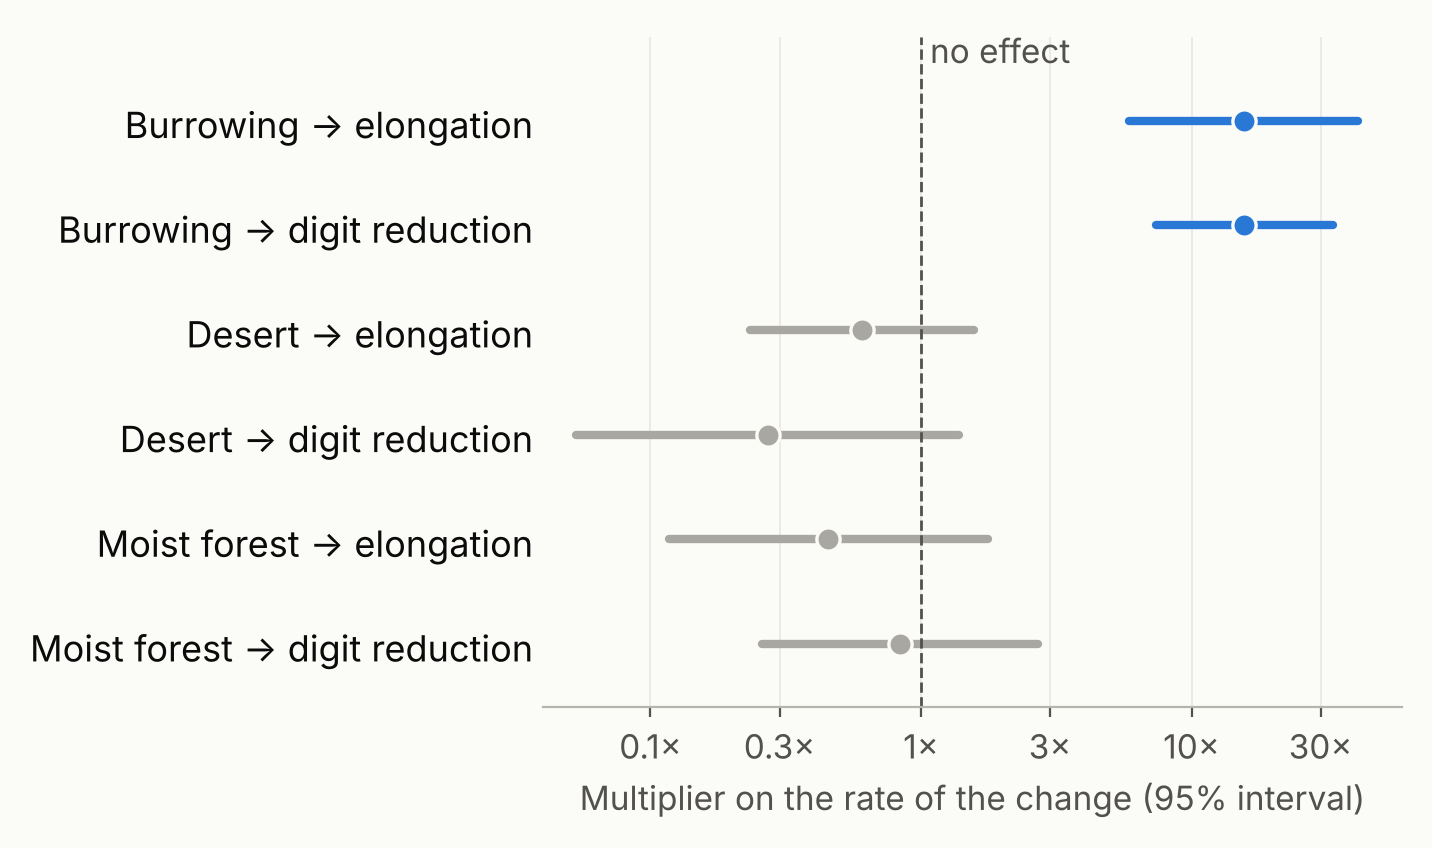
\includegraphics[width=0.62\textwidth]{figures/drivers.png}
\caption{How much each environment multiplies the rate of each body change, with 95\% intervals. A value of 1 means no effect. Only burrowing (blue) clearly speeds the changes; for deserts and moist forests every interval includes no effect.}
\label{fig:drivers}
\end{figure}

\section{How sure are we?}

Every number above comes with a range, a \emph{95\% interval}, that expresses how much it could reasonably vary. We built these ranges in two ways. For the network, we rebuilt it 200 times, each time from a random 80\% of the species, and redid the analysis; the same bottleneck appeared all 200 times, with conductance between 0.002 and 0.004. For the evolutionary model, we drew many alternative sets of the 15 numbers that fit the data almost as well as the best one, and repeated the reconstructions and walks for each. This gives, for example, a waiting time of 447 to 566 million years before a lineage starts, a finishing time of 33 to 41 million years, 43 to 54 separate origins, a walk speedup of 2.4 to 2.8 times, and a what-if effect of 18 to 31\% for doubling burrowing. Finally, we repeated the network analysis on a different published family tree (Zheng and Wiens 2016) and with snakes included, and found the same bottleneck both times.

\section{The big picture}

Snake-like bodies are hard to start and quick to finish. A strong barrier keeps the great majority of lizard lineages in the ordinary four-legged design, which is why the snake-like body is rare. But each step toward it makes the next one easier, so the few lineages that start, usually by moving underground, tend to finish the journey quickly and end up in the same place. That is why the design keeps reappearing in unrelated families, and why so few species are caught halfway. In network terms, evolution's traffic flows downhill toward the snake-like side, through a single narrow passage that almost nobody stops in.

The broader point is methodological. Tools built to study social networks and the internet, such as small-world measures, spectral bottlenecks and random walks, can also map evolution itself: its roads, its narrow passages, how fast traffic moves and which way it flows. Because the method needs only a family tree and a few measurements, it could be applied to other designs that nature keeps reinventing, such as the many unrelated crustaceans that have evolved crab-like bodies.

\section{Limitations and next steps}

Our picture simplifies in several ways. We reduce bodies to four yes-or-no features, which hides gradual change; finger and toe counts are still missing for about 500 lizards; our ranges rely on a statistical approximation; habitat categories are coarse; and the scenarios show what the patterns imply rather than what will actually happen. Next we plan to repeat the analysis on 100 alternative family trees, replace the yes-or-no features with actual counts so the map of body plans has hundreds of nodes rather than twelve, test climate measurements as drivers, and apply the method to a second group of animals.

\section*{Glossary}

\small
\begin{tabularx}{\textwidth}{@{}lX@{}}
\toprule
Body plan & A combination of our four yes-or-no features; one node of the map in Figure~\ref{fig:bodyplans}. \\
Bottleneck & A thin place in a network, where few edges cross between two large groups. \\
Cheeger cut & The low-conductance split found by the spectral method, with a guarantee from Cheeger's inequality. \\
Clustering coefficient & How often two neighbors of a node are also neighbors of each other. \\
Conductance & Edge weight crossing a split divided by edge weight on its smaller side; near 0 means a bottleneck. \\
Convergence & Unrelated lineages independently evolving the same design. \\
Convergence link & An edge between two look-alike, snake-ward species whose lineages split over 100 million years ago. \\
Fiedler vector & The second eigenvector of the graph Laplacian; nodes on the same side of a bottleneck get similar values. \\
Graph, node, edge & A network; its dots; its lines. \\
Hitting time & The expected number of steps a random walk needs to reach a target. \\
Likelihood & How probable a model's settings make the observed data; fitting maximizes it. \\
Lineage & One line of descent through time. \\
Markov chain & A random process in which the next move depends only on the current state. \\
Phylogeny & The family tree of species, with branch lengths in time. \\
Random walk & A wanderer moving between neighboring nodes at random; biased if some moves are favored. \\
Small world & A network that is highly clustered yet has short paths, thanks to a few long-range shortcuts. \\
Stochastic mapping & Generating plausible full histories of change on a tree that agree with today's data. \\
95\% interval & A range that the true value falls in with high confidence, given the data and model. \\
\bottomrule
\end{tabularx}

\normalsize
\section*{References}
{\small
Bergmann, P.\,J.\ and Morinaga, G.\ (2019). The convergent evolution of snake-like forms by divergent evolutionary pathways in squamate reptiles. \textit{Evolution}.\par
Camaiti, M.\ et al.\ (2022). A database of the morphology, ecology and literature of the world's limb-reduced skinks. \textit{Journal of Biogeography} 49, 1397--1406.\par
Chung, F.\ (1997). \textit{Spectral Graph Theory}. American Mathematical Society.\par
Meiri, S.\ (2024). SquamBase: a database of squamate (Reptilia: Squamata) traits. \textit{Global Ecology and Biogeography} 33.\par
Nielsen, R.\ (2002). Mapping mutations on phylogenies. \textit{Systematic Biology} 51, 729--739.\par
Pagel, M.\ (1994). Detecting correlated evolution on phylogenies. \textit{Proceedings of the Royal Society B} 255, 37--45.\par
Title, P.\,O.\ et al.\ (2024). The macroevolutionary singularity of snakes. \textit{Science}.\par
Watts, D.\,J.\ and Strogatz, S.\,H.\ (1998). Collective dynamics of small-world networks. \textit{Nature} 393, 440--442.\par
Zheng, Y.\ and Wiens, J.\,J.\ (2016). Combining phylogenomic and supermatrix approaches, and a time-calibrated phylogeny for squamate reptiles based on 52 genes and 4162 species. \textit{Molecular Phylogenetics and Evolution} 94, 537--547.\par
}

\end{document}
